\section{Mravenčí kolonie}
Algoritmus popsaný začátkem 90. let známý pod jménem Optimalizace mravenčí kolonií patří do kategorie hejnových algoritmů. \cite{Colorni1991} Jedná se o heuristickou metodu hledání nejkratší cesty. Velká výhoda tohoto algoritmu spočívá v jeho adaptabilitě. Dá se využít v prostředí, kde v průběhu času možné cesty zaníkají a vznikají nové. 
\par
Přestože má každý jedinec definované základní možnosti, chování celého mraveniště je velmi strukturované. Jedná se o výsledek koordinovaných iterací. Tato práce zkouší využít algoritmus pro navigaci agentů místo pro optimalizaci nejkratší cesty. 

\subsection{Popis metody}
Jednotliví agenti (mravenci) putují nahodile po okolí mraveniště. Jakmile naleznou potravu, vrací se do mraveniště stejnou cestou jakou k potravě dorazili. Po cestě zpátky za sebou zanechávají feromonovou stopu. Pokud jiný mravenec tuto stopu zachytí, je větší pravděpodobnost, že se vydá cestou feromonu než náhodnou. Mravenec $k$ ve vrcholu $i$, grafu $G = (N, A)$ se přesune do sousedního vrcholu $j$ s pravděpodobností $p_{ij}^k$:  
\begin{equation*}
p_{ij}(t) = \frac{[\tau_{ij}(t)^\alpha] [\eta_{ij}]\beta}{\sum\limits_{j=1}^n{[\tau_{ij}(t)^\alpha] [\eta_{ij}]\beta}},
\end{equation*}
kde $N_i^k$ představuje množinu všech vrcholů dostupných mravenci $k$. Koeficienty $\alpha$, $\beta$ a $\rho$ jsou obecnými parametry algoritmu \cite{Blum2005}. 
\par
Feromon postupně vyprchává, takže jakmile potrava zanikne, postupně zanikne i feromonová stopa a mravenci začnou zase náhodně prohledávat. Každou iteraci se každá feromonová stopa upraví podle vztahu:
\begin{equation*}
\tau_{ij} = (1 - \rho)\tau_{ij}.
\end{equation*}

\subsection{Alternativní využití}
V rámci projektu byl tento algoritmus lehce upraven pro potřebu navigace agentů. Nejprve byla odebrána nutnost grafu. Mravenci se pohybovali zcela náhodně po mapě, kdy každý mravenec ušel náhodnou vzdálenost v definovaném intervalu a poté se náhodně rozhodl kterým směrem půjde příště. Směr, který si mohl mravenec vybrat byl omezen intervalem úhlu jeho vidění. 
\par
Každý mravenec měl definováno jak dlouho vydrží hledat potravu či feromonovou stopu. Po uplynutí této doby se musí vrátit do mraveniště a začít hledat znovu. Tímto bylo zamezeno, aby se mravenec vzdálil od mraveniště příliž daleko a aby jeho cesta k potravě byla co možná nejkratší. 
\begin{figure}[H]
	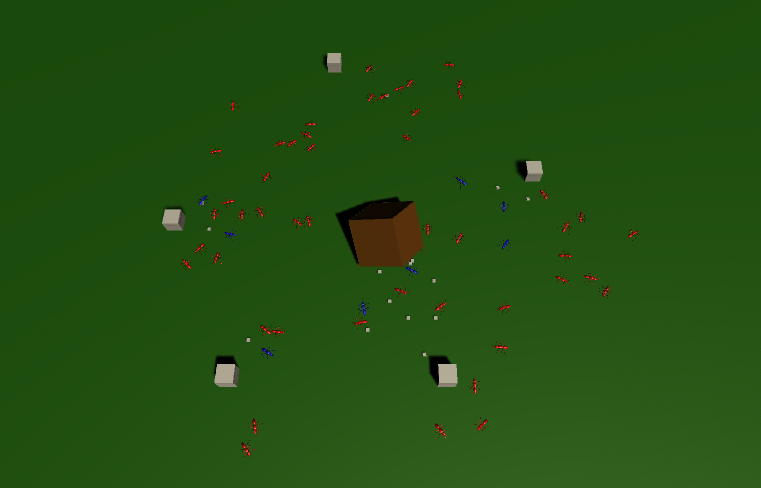
\includegraphics[width=10cm]{antcolony.png}
	\centering
	\caption{Implementovaný model mravenčí kolonie v průběhu simulace}
	\label{fig:antcolony}
\end{figure}
Na obrázku \ref{fig:antcolony} lze vidět uprostřed mraveniště, kolem kterého je rozmístěno 5 bílých krychlí představující potravu. Mravenci, kteří potravu nalezli a vracejí se do mraveniště jsou označeni modrou barvou, zatímco červení mravenci potravu teprve hledají. 